
\chapter{Die Programmiersprache Rust}

%Rust ist eine Programmiersprache, die versucht performante -- und daher durch Abstraktionen mit keinem zusätzlichen \enquote{Kosten} \todo{ref zero cost abstractions} -- und sichere Programmierung zu ermöglichen.
Rust hat als Ziel, eine sichere (siehe \autoref{rust:guarantees}) und performante Systemprogrammiersprache zu sei.
Abstraktionen sollen die Sicherheit, Lesbarkeit und Nutzbarkeit verbessern aber keine unnötigen Performanceeinbußen verursachen (siehe \autoref{rust:zero_cost}).

Aus anderen Programmiersprachen bekannte Fehlerquellen -- wie \enquote{dangling pointers}, \enquote{double free} oder \enquote{memory leaks} --  werden durch strikte Regeln und mit Hilfe des Compilers verhindert (\autoref{rust:guarantees}).
Im Gegensatz zu Programmiersprachen, die dies mit Hilfe ihrer Laufzeitumgebung\footnote{u.a. Java Virtual Maschine (JVM), Common Language Runtime (CLR)} sicherstellen, werden diese Regeln in Rust durch eine statische Lebenszeitanalyse (\autoref{rust:static_analysis}) und mit dem Eigentümerprinzip (\autoref{rust:ownership}) bei der Compilation überprüft und erzwungen.

Diese erlaubt Rust eine zur Laufzeit hohe Ausführgeschwindigkeit zu erreichen.
Das Eigentümerprinzip (siehe \autoref{rust:ownership}) und die Markierung durch von Datentypen durch Merkmale (siehe \autoref{rust:traits}) vereinfacht es, nebenläufige und sichere Programme zu schreiben.

Rust hat in den letzten Jahren viel an Beliebtheit gewonnen und ist 2018 das dritte Jahr in Folge als beliebteste Programmiersprache in einer Umfrage auf Stack Overflow gewählt worden \cite{rust:stack_overflow:mose_loved}.
Rust scheint dem Anspruch, eine sichere und performante Programmiersprache zu sein, gerecht zu werden:

\begin{quotation}
	\textit{\enquote{Again, Rust guides you toward good programs}}
	\cite[497]{rust:orly_programming}
\end{quotation}

\begin{quotation}
	\textit{\enquote{[..]Leute, die [..] sichere Programmierung haben wollen, [..] können das bei Rust haben, ohne [..] undeterministischen Laufzeiten oder Abstraktionskosten schlucken zu müssen. }}
	\cite[Felix von Leitner in einem Blogeintrag]{rust:fefe}
\end{quotation}

\begin{quotation}
	\textit{\enquote{[..] Rust makes it safe, and  provides nice tools}} 
	\cite[Folie 130, Federico Mena-Quintero in \enquote{Ersetzen von C Bibliotheken durch Rust}]{rust:c_is_hostile_mena}
\end{quotation}

\begin{quotation}
	\textit{\enquote{Rust hilft beim Fehlervermeiden}} 
	\cite[Federico Mena-Quintero in einem Interview]{rust:c_is_hostile_golem}
\end{quotation}

\begin{quotation}
	\textit{\enquote{Rust is [..] a language that cares about very tight control}}
	\cite[Diskussion zwischen Programmierern auf Reddit]{rust:tight_control}
\end{quotation}


%Durch Merkmale (siehe \autoref{rust:traits}) kann die Zugriffsart auf Datentypen über verschiedene Threads hinweg festgelegt oder verhindert werden, wodurch falsche nebenläufige Programmierung zur Compilezeit erkannt und verhindert wird.
%Dies begünstigt parallelisierte Architekturen und ermöglicht es, die vielen CPU-Kerne auf modernen Computern einfacher zu nutzen.
%\todo{rust performance very wow, much parallel, great safety}

%Programmierer müssen sich für Rust an ein striktes Regelwerk und einen \enquote{besorgten} Compiler (siehe \autoref{rust:worried_compiler}) gewöhnen, erhalten im Gegenzug aber eine Sprache, die ein undefiniertes Verhalten nur in absoluten Ausnahmefällen kennt (siehe \autoref{rust:undefined}).
%Eine vom Compiler bemängelte Formatierung des Programmcodes und Benennung von Datentypen, Felder und Funktionen (siehe \autoref{rust:styleguide}) erlaubt ein einheitliches Auftreten des Programmcodes innerhalb der \todo{Community}.

%\todo{rust sehr sauber, nahezu nix undefined (ref), nix uninitalized access(ref), datentypen namen u/i..(ref), styleguide}


\clearpage
\section{Geschichte}
\label{rust:history}

In 2006 begann Graydon Hoare die Programmiersprache Rust in seiner Freizeit als Hobbyprojekt zu entwickeln \cite{rust:faq}.
Als Grund nannte er seine Unzufriedenheit mit der Programmiersprache C++, in der es sehr schwierig sei, fehlerfreien, speichersicheren und nebenläufigen Programmcode zu entwickeln.
Zudem beschrieb er C++ als \enquote{ziemlich fehlerträchtig} \cite{rust:heise_interview_graydon}.

Auch Federico Mena-Quintero -- Mitbegründer des GNOME-Projekts \cite{rust:gnome:federico}  --
äußerte in einem Interview mit Golem im Juli 2017 seine Bedenken an der Verwendung der \enquote{feindseligen} Sprache C \cite{rust:c_is_hostile_golem}.
In Vorträgen vermittelt er seither, wie Bibliotheken durch Implementationen in Rust ersetzt werden können \cite{rust:c_is_hostile_mena}.

Ab 2009 begann Mozilla die Weiterentwicklung finanziell zu fördern, als einfache Tests und die Kernprinzipien demonstriert werden konnten.
Die Entwicklung der Programmiersprache, des Compilers, des Buchs, von Cargo, von crates.io und von weiteren Bestandteilen findet öffentlich einsehbar auf \gls{github}  unter \url{https://github.com/rust-lang} statt und wird nicht ausschließlich von Mozilla Angestellten koordiniert.
Dadurch kann sich jeder an Diskussionen oder Implementation beteiligen, seine Bedenken äußern oder Verbesserungen vorschlagen.

Durch automatisierte Tests (siehe \autoref{rust:tests}) in Kombination mit drei Veröffentlichungskanälen (\enquote{relese}, \enquote{stable} und \enquote{nightly}) und \enquote{feature gates} (siehe \autoref{rust:feature_gates}) wird die Stabilität des Compilers und die der Standardbibliothek (\autoref{rust:stdlib}) gewährleistet.

Rust ist wahlweise unter MIT oder der Apache Lizenz in Version 2 verfügbar \cite{rust:copyright}.

\section{Anwendungsgebiet}

Das Ziel von Rust ist es, das Designen und Implementieren von sicheren und nebenläufigen Programmen möglich zu machen.
Gleichzeitig soll der Spagat geschaffen werden, nicht nur ein sicheres aber lediglich theoretisches Konstrukt zu sein, sondern  in der Praxis eine Anwendung zu finden.
Als Beweis könnte hierbei auf die Umstellung von Firefox auf Rust und Servo -- ein minimaler Webbrowser komplett in Rust geschrieben -- verwiesen werden \cite{rust:faq}.

Interessant ist eine Diskussion von 2009, bei der \enquote{sicher aber nutzlos} und \enquote{unsicher aber brauchbar} Gegenübergestellt wurde.
Programmiersprachen scheinen auf der Suche nach dem nicht existierende \enquote{Nirvana} zu sein, das sowohl sichere als auch brauchbare Programmierung verspricht \cite[ab ca Minute 58:20]{rust:infoq:null}.
Rust möchte dieses Nirvana gefunden haben.
% bei einer Diskussion \footnote{Siehe auch \enquote{unsafe but useful}/\enquote{safe but useless} \cite[ab ca Minute 58:20]{rust:infoq:null}}.

\subsection{Kompatibilität}
Da Rust den \gls{llvm}-Compiler nutzt, erbt Rust auch eine große Anzahl der Zielplattformen die \gls{llvm} unterstützt.
Die Zielplattformen sind in drei Stufen unterteilt, bei denen verschieden stark ausgeprägte Garantien vergeben werden. Es wird zwischen
\begin{itemize}
	\item \enquote{Stufe 1: Funktioniert garantiert} (u.a. X86, X86-64),
	\item \enquote{Stufe 2: Compiliert garantiert} (u.a. ARM, PowerPC, PowerPC-64) und
	\item \enquote{Stufe 3} (u. a. Thumb (Cortex-Microcontroller))
\end{itemize}
unterschieden \cite{rust:platform_support}.
Diese Unterscheidung wirkt sich auch auf die Stabilisierungsphase und Implementation neuer Funktionen aus (Beispiel \enquote{128-bit Integer Support} \cite{rust:github:128bit_integer}).

\subsection{Veröffentlichungszyklus}
\label{rust:feature_gates}

Es stehen Versionen in drei verschieden Veröffentlichungskanälen zur Verfügung:
\begin{itemize}
	\item \textbf{nightly}:
	Version die einmal am Tag mit dem aktuellen Stand des Quellcodes gebaut wird.
	Experimentelle und nicht fertige Features sind hier zwar enthalten, aber hinter \enquote{feature gates} versteckt.
	Diese können durch ein entsprechendes Attribute (siehe \autoref{rust:attributes}) geöffnet werden (\rustcinline{#[feature(const_fn)]} ermöglicht die Definition von Konstante Funktionen, Stand \today).
	
	\item \textbf{beta}: Alle sechs Wochen wird die aktuellste Nightly zur Beta befördert und es werden nur noch Fehler aus dieser Version getilgt.
	Dieser Prozess könnte auch als Reifephase bezeichnet werden.
	\item \textbf{stable}: Nach sechs Wochen wird die aktuellste Beta zur Stable befördert und veröffentlicht.
	Gleichzeitig wird auch eine neue Beta veröffentlicht.
\end{itemize}

\subsection{Ökosystem}

Mit Rust wird nicht nur eine Programmiersprache, sondern auch ein umfassendes Ökosystem angeboten.

Cargo ist vermutlich das größte angebotene Werkzeug.
Es löst Abhängigkeiten auf, indem es auf das öffentliche Verzeichnis unter \url{https://crates.io} zurückgreift und diese entsprechend herunterlädt und compiliert.
Zum jetzigen Zeitpunkt (\today) sind über 14.000 Crates öffentliche erreichbar und nutzbar.
Zudem wird durch Crago eine \textit{Cargo.toml} verlangt, in der Metainformationen einer Crate hinterlegt sind.
Dies Umfasst u.a. Name, Version, Autor, Lizenz und Abhängigkeiten.

Eine Crate kan von jedem veröffentlicht werden, insofern derjenige ein \gls{github}-Konto besitzt, der Name der Crate noch nicht vergeben ist und der Programmcode compiliert.
Die API-Dokumentation der jeweiligen Crate wird dabei automatisiert auf \url{https://docs.rs} veröffentlicht.

Unter \url{https://www.rust-lang.org} ist die Website von Rust erreichbar und unter \url{https://doc.rust-lang.org} sowohl die API-Dokumentation der Standardbibliothek als auch as Hauseigene Rust Buch in Version 1 und 2.
Die Entwicklung findet dagegen auf \gls{github} unter \url{https://github.com/rust-lang} statt.

Kleine Testprogramme und Experimente können auf dem \enquote{Spielplatz} unter \url{https://play.rust-lang.org} compiliert und ausgeführt werden, ohne lokal etwas zu installieren.


\section{Aufbau eines Projektverzeichnisses}

Der Aufbau eines Rust Projektverzeichnis kann zwischen zwei verschiedenen Arten differenziert werden.
Zum einen gibt es den klassische Aufbau, in dem lediglich der Programmcode liegt und der Compiler direkt aufgerufen und parametrisiert wird.
Zum anderen wird der Aufbau als Crate (siehe \autoref{rust:structure:crate}) empfohlen, da dadurch Abhängigkeiten automatisch aufgelöst werden können aber auch Metainformationen bezüglich des Autors, der Version und der Abhängigkeiten hinterlegt werden müssen.
Ein klassischer Aufbau ist dagegen nur selten anzutreffen.


\subsection{Klassisch}
\label{rust:structure:classic}
\begin{wrapfigure}{l}[-1em]{.5\textwidth}
	\rustcinclude
		{rust:structure:classi}
		{Verzeichnisstruktur des Quelltext-Verzeichnisses}
		{sections/rust.classic.txt}
\end{wrapfigure}

Das Quelldatei-Verzeichnis sollte entweder eine \textit{main.rs} für Ausführbare Programme oder eine \textit{lib.rs} für Bibliotheken enthalten.
Während der Paketmanager Cargo eine solche Benennung als Standardkonvention erwartet, kann bei manueller Nutzung des Compilers auch ein anderer Name für die Quelldatei vergeben werden.

Der Compiler startet in der Wurzeldatei und lädt weitere Module, die durch \rustcinline{mod module;} gekennzeichnet sind (ähnlich \ccinline{# include "module.h"} in C/C++).
Ein Modul kann dabei eine weitere Quelldatei oder ein ganzes Verzeichnis sein.
Ein Verzeichnis wird aber nur als gültiges Modul interpretiert, wenn sich eine \textit{mod.rs} Datei darin befindet.
Um Datentypen und Funktionen aus einem Modul nutzen zu können, ohne dessen kompletten Pfad jedes mal auszuschreiben, müssen sie durch zum Beispiel \rustcinline{use module::functionality::Data;} in dem aktuellen Namensraum bekannt gemacht werden.

Wie bereits angedeutet, wird in Rust nicht eine \enquote{Klasse}, Datenstruktur oder Aufzählung pro Datei erwartet, sondern eine Quelldatei entspricht einem Modul.
Diese Umfasst in vielen fällen wenige aber mehrere Datenstrukturen, zugehörige Aufzählung und Fehlertypen.
%Module (Verzeichnisse oder Quelldateien) gesucht wird. , in der Module durch \rustcinline{mod module;} und Quelldateien durch \rustcinline{mod functionality;} \enquote{inkludiert} werden können.
%Eine Datei \textit{mod.rs} ist die Wurzeldatei eines Moduls.

\subsection{Als Crate}
\label{rust:structure:crate}

\begin{wrapfigure}{r}{.4\textwidth}
	\rustcincludeml
		{rust:structure:cargo}
		{Vereinfachte Verzeichnisstruktur einer \enquote{crate}}
		{sections/rust.cargo.txt}
\end{wrapfigure}



Eine \enquote{Crate} (dt. Kiste/Kasten) erweitert den klassischen Aufbau um eine \textit{Cargo.toml} Datei, in der Metainformationen zum Projekt hinterlegt werden.
Durch die Benutzung des Werkzeugs \enquote{Cargo} (dt. Fracht/Ladung) können Abhängigkeiten automatisch aufgelöst, heruntergeladen und compiliert werden.

Eine Crate kann entweder ein ausführbares Programm oder eine Bibliothek sein.
Davon abhängig is die Wurzeldatei \textit{src/main.rs} (für ein ausführbares Programm) oder \textit{src/lib.rs} (für eine Bibliothek).
Mit dem erzeuge einer Crate (\rustcinline{cargo new --bin meinProg} bzw. \rustcinline{cargo new --lib meineBib}) wird auch gleichzeitig \gls{git} für das Verzeichnis initialisiert.

\section{Hello World}


\begin{wrapfigure}{l}{.5\textwidth}
	\rustcinclude
		{rust:hello_world}
		{\enquote{Hello World} in Rust}
		{sections/rust.hello_world.rs}
\end{wrapfigure}

Der Programmcode in \autoref{rust:hello_world} gibt auf der Konsole \monospaceinline{Hello World} aus.
Das \rustcinline{fn} die Funktion \rustcinline{main} definiert und diese der Startpunkt des Programms ist, wird vermutlich wenig überraschend sein.
Viel überraschender ist vermutlich eher das Ausrufezeichen in Zeile 2, da es auf den ersten Blick dort nicht hingehören sollte.
In Rust haben Ausrufezeichen und Fragezeichen besondere Bedeutungen, weswegen die Verwendung in Zeile 2 trotzdem richtig ist.

Die Bedeutung des Fragezeichens dient zum schnelleren Auswerten von \rustcinline{Rusult<_, _>}-Werten und wird in \autoref{rust:result} genauer erklärt.
Das Ausrufezeichen kennzeichnet, dass der ansonsten augenscheinliche Funktionsaufruf tatsächlich ein Aufruf einer Makrofunktion ist.

Eine Funktion \rustcinline{println} gibt es nicht, auch keine aus C erwarteten Funktionen wie \ccinline{printf}, \ccinline{fputs} oder \ccinline{sprintf}.
Eine Ausgabe erfolgt durch das \rustcinline{println!} Makro, welches eine String durch Nutzung des \rustcinline{format!} Makros formatiert und erstellt.
Daraufhin wird das \rustcinline{writeln!} Makro verwendet, um die formatierte Zeichenkette auf die Standardausgabe zu schreiben.

\section{Einfache Datentypen}
\label{rust:types:simple}

Die Datentypen in Rust sind im wesentlichen die üblichen  Verdächtigen: \rustcinline{bool} für boolische Ausdrücke; \rustcinline{char} für ein einzelnes Unicode Zeichen; \rustcinline{str} für eine Zeichenkette; \rustcinline{u8}, \rustcinline{i8}, \rustcinline{u16}, \rustcinline{i16}, \rustcinline{u32}, \rustcinline{i32}, \rustcinline{u64}, \rustcinline{i64}, (bald \rustcinline{u128}, \rustcinline{i128} \cite{rust:github:128bit_integer:rfc}) und \rustcinline{usize}, \rustcinline{isize}  für ganzzahlige Werte; \rustcinline{f32}, \rustcinline{f64} für Fließkommazahlen in einfacher und zweifacher Präzision; Arrays und Slices \cite{rust:book:primitives}.

Ganzzahlige Datentypen mit einem führenden \rustcinline{u} sind vorzeichenlos (\enquote{unsigned}), vorzeichenbehaftete (\enquote{signed}) sind dagegen mit einem \rustcinline{i} gekennzeichnet.
Die darauf folgende Zahl gibt die Anzahl der Bits wieder, die der Datentyp groß ist.
Die einzige Ausnahme bildet unter den ganzzahligen Datentypen ist \rustcinline{usize} bzw \rustcinline{isize}, da dieser immer so groß ist, wie die Architektur der Zielplattform.
Bei der Indexierung eines Arrays bzw. einer Slice würde ein Datentyp, mit einer global definierten Größe, keinen Sinn ergeben. Das Maximum an adressierbaren Einträgen ist von der Architektur der Zielplattform abhängig.
Fließkommazahlen sind mit einem führenden \rustcinline{f} gekennzeichnet.

Durch dieses Schema bei der Bezeichnung der Datentypen wird eine Verwirrung wie zum Beispiel in C unterbunden, wo die primitiven Datentypen (\ccinline{short}, \ccinline{int}, \ccinline{long}, ..) keine definierte Größe haben, sondern dies abhängig vom eingesetzten Compiler und der Zielplattform ist \cite[187]{deitel2013c}. Erst ab C99 wurden zusätzliche, aber optionale, ganzzahlige Datentypen mit bestimmten Größe definiert \cite[141]{goll2014c}.

Konstanten können eindeutig einem Datentyp zugewiesen werden, indem dieser angehängt wird: \rustcinline{4711u16} ist vom Datentyp \rustcinline{u16}.
Des weiteren dürfen Ziffern durch beliebiges setzen von \rustcinline{_} getrennt werden, um die Lesbarkeit zu erhöhen: \rustcinline{1_000_000_f32}.
Eine Schreibweise in Binär (\rustcinline{0b0000_1000_u8}), in Hexadezimal (\rustcinline{0xFF_08_u16}) oder Oktal (\rustcinline{0o64_u8}) ist auch möglich. 
Konstante Zeichen und Zeichenketten können auch automatisch in Bytes gewandelt werden (\rustcinline{b'b'} entspricht \rustcinline{0x62_u8} und \rustcinline{b"abc"} entsricht \rustcinline{&[0x61_u8, 0x62_u8, 0x63_u8]}).

Arrays haben immer eine zur Compilezeit bekannte Größe und müssen auch immer mit einem Wert initialisiert werden (siehe \autoref{rust:no_unitialized_usage}).
Dynamische Arrays auf dem Stack gibt es (noch? \cite{rust:github:alloca}) nicht,
stattdessen wird auf die Vektor Implementation der Standardbibliothek verwiesen (siehe \autoref{rust:stdlib}).
Die Notation für Arrays ist \rustcinline{[<Füllwert>; <Größe>]}, wobei die Größe ein konstanter Wert sein muss.
\rustcinline{[0_u8; 128]} steht demnach für ein 128 Byte langes Array, das mit 0-en vom Datentyp \rustcinline{u8} gefüllt ist.

\enquote{Slices} (dt. Scheiben/Stücke) bezeichnet Rust Referenzen oder Referenzen auf Teilbereiche von Arrays und Slices.
Die Größe einer Slice wird dabei mit der Referenz auf die Startposition gespeichert und oft auch \enquote{fat pointer} genannt.
Ein zusätzlicher Parameter für die Größe eines Buffers, wie in C üblich, ist somit unnötig.
Die Notation ähnelt dabei die eines Arrays, aber ohne Größenspezifikation: \rustcinline{&[<Datentyp>]}.
Eine Slice ist immer eine Referenz.
Um eine Slice auf ein Array oder eine andere Slice zu erhalten, muss der Start- und  Endindex des Teilbereiches angegeben werden.
Falls kein Start- oder Endindex angegeben wurde, wird das jeweilige Limit übernommen.

\todo{let, let mut, let ... : type = ..., \& \&mut, deref via *}

https://www.youtube.com/watch?v=-Tj8Q12DaEQ \\
\todo{static type system with local type inference } \\

Folgendes Beispiel soll die Notation von Arrays und Slices Beispielhaft verdeutlichen:

\rustcinclude
	{rust:slices:example}
	{Beispiel eines Arrays und einer Slice}
	{sections/rust.slices.rs}
	
Das in \autoref{rust:slices:example} gezeigte Programm, gibt auf der Konsole \rustcinline{2, 3, 4, } aus.

\section{Zusammengesetzen Datentypen}
\label{rust:types:composed}

Die Programmiersprache Rust kennt neben den einfachen Datentypen (\autoref{rust:types:simple}) weitere Möglichkeiten Daten zu organisieren:
\begin{itemize}
	\item ein Tupel, das mehrere Werte namenlos zusammenfasst: \rustcinline{(f32, u8)}: \rustcinline{a.0 = 1.0_f32},
	\item eine Datenstruktur, die wie in C Datentypen namenbehaftet zusammenfasst: \linebreak\rustcinline{struct Punkt \{ x: f32, y: f32 \} }: \rustcinline{p.x = 1.0_f32},
	\item und Aufzählungen: \rustcinline{enum Bildschirm \{ Tv, Monitor, Leinwand \}}.
\end{itemize}

Im Vergleich zu C kann ein Eintrag in einem \rustcinline{enum} gleichzeitig Daten wie eine Datenstruktur oder ein Tupel halten, oder lediglich einen Ganzzahlwert repräsentieren.
Mit dem \rustcinline{type} Schlüsselwort können Aliase erstellt oder im Falle von FFI (siehe \autoref{rust:ffi}) aufgelöst werden: \rustcinline{type Vektor = (f32, f32);}
Felder einer Struktur können zudem mit \rustcinline{pub} oder \rustcinline{pub(crate)} gekennzeichnet werden (siehe \autoref{rust:access_modifier}).

Seit Version 1.19 ist auch der Datentyp \rustcinline{union} in Rust verfügbar \cite{rust:v1.19}.
Eine \rustcinline{union} kann aber nur in \rustcinline{unsafe}-Blöcken verwendet werden, da der Compiler eine Ordnungsgemäße Nutzung nicht überprüfen kann.
Für diese Abschlussarbeit hat der Datentyp aber keine Relevanz und wird daher nicht weiter erwähnt.

\section{Funktionen, Ausdrücke und Statements}

Funktionen werden durch \rustcinline{fn} gekennzeichnet, gefolgt mit dem Funktionsnamen, der Parameterliste und zuletzt der Datentyp für den Rückgabewert.
Selbst wenn kein expliziter Rückgabetyp angegeben wird, wird formal \rustcinline{()} zurück gegeben; \rustcinline{()} entspricht etwa \ccinline{void} aus bekannten Programmiersprachen.
Die Parameterliste unterscheidet sich von bekannten Programmiersprachen wie C und Java, indem zuerst der Variablenname und darauf folgend der Datentyp notiert wird.

\rustcinclude
	{rust:fn:add}
	{Beispiel einer Funktion}
	{sections/rust.fn.add.rs}
	
Obwohl in Zeile 2 von \autoref{rust:fn:add} kein \rustcinline{return} zu sehen ist, wird trotzdem das Ergebnis der Addition zurückgegeben.
Dies liegt daran, da in Rust vieles ein Ausdruck ist und somit einen Rückgabewerte liefert \cite{rust:book:statements}.
Auch ein if-else ist ein Ausdruck und kann einen Rückgabewert haben.
Ein bedingter Operator (?:) is somit unnötig, da stattdessen ein if-else verwendet werden kann: \rustcinline{let a = if b \{ c \} else \{ d \};}. 
Auch eine Zeile mit einen Semikolon hat formal einen Rückgabewert: \rustcinline{()}.

\section{Implementierung einer Datenstruktur}

Zu einer Datenstruktur oder Aufzählung kann ein individuelles Verhalten implementiert werden.
In dieser Kombination ähneln diese Konstrukte sehr einer Klasse aus bekannten objektorientierten Programmiersprachen, wie zum Beispiel Java, C\# oder C++ (siehe auch \autoref{rust:oop}).

Einen Konstruktor gibt es jedoch nicht; lediglich die Konvention, eine statische Funktion \rustcinline{new} stattdessen zu verwenden \cite{rust:book:constructors}:

\rustcinclude
	{rust:struct:impl}
	{Punkt Datenstruktur mit einem \enquote{Konstruktor}}
	{sections/rust.struct.impl.rs}
	
In seltenen Fällen wird auch \rustcinline{Default} implementiert (siehe \autoref{rust:trait:default}), wodurch eine statische Funktion \rustcinline{default()} als Konstruktor ohne Parameter bereitgestellt wird.

Da eine Funktionsüberladung nicht möglich ist, soll bei weiteren Konstruktoren ein sprechender Name verwendet werden.
Der \rustcinline{Vec<_>} der Standardbibliothek (siehe \autoref{rust:stdlib}) bietet zum Beispiel zusätzlich \rustcinline{Vec::with_capacity(capacity: usize)} an, um einen Vektor mit einer bestimmten Größe zu initialisieren.

Für Funktionen können auch die Zugriffsmodifikatoren festgelegt werden (siehe \autoref{rust:access_modifier}). 

\section{Generalisierung durch Traits}
\label{rust:traits}
\label{rust:generics}
\label{rust:trait:default}

Ähnlich wie Java oder C\# bietet Rust durch einen eigenen Typ die Möglichkeit, ein gewünschtes Erscheinungsbild zu generalisieren, ohne gleichzeitig eine Implementation vorzugeben.
Im Rust wird dieser Typ \enquote{Trait} (dt. Merkmal) genannt.

Für Merkmale werden Funktionen in einem entsprechenden \rustcinline{trait <Name> \{ \}} Block ohne Rumpf deklariert.
Optional kann auch ein Standardrumpf implementiert werden, der bei einer Spezialisierung überschrieben werden darf.
Auch auf ein Merkmal kann ein Zugriffsmodifikatoren gesetzt werden (siehe \autoref{rust:access_modifier}).

Die Implementation eines Merkmals wird für jeden Datentyp in einem separaten Block vorgenommen und entspricht der Notation \rustcinline{impl Merkmal for Datentyp \{ fn ... \} }.
Alternativ können Implementationen auch für ganze Gruppen von anderen Merkmalen vorgenommen werden: \rustcinline{impl<T> Merkmal for T where T: Clone \{ ... \} } (entspricht: \enquote{implementiere \rustcinline{Merkmal} für alle, die \rustcinline{Clone}-bar sind}).

In Zukunft -- oder jetzt in \enquote{nightly} und hinter dem \enquote{feature gate} \rustcinline{specialization} -- wird es möglich sein, ein Standardverhalten für Gruppen zu implementieren und dieses später, für einen spezialisierten Fall, zu überschreiben \cite{rust:github:specialization}.

Merkmale unterscheiden sich in ihrer Handhabung gegenüber anderen Datentypen, da sie im allgemeinen keine bekannte Größe zur Compilezeit haben.
Während dies in Programmiersprachen wie Java und C\# automatisch durch die Darstellung abstrahiert und versteckt wird, hat ein Entwickler in Rust mehr Kontrolle über die Handhabung.

Dabei gibt es mehrere Vorgehensweisen:
\begin{itemize}
	\item Die einfachste Art erfolgt über das Leihen mittels Referenz: \rustcinline{fn foo(bar: \&Bar)} oder \rustcinline{fn foo(bar: \&mut Bar)} -- ein Unterschied zu anderen Datentypen ist nicht zu erkennen.
	Hierbei werden Funktionen aber dynamisch über eine \enquote{vtable} aufgerufen, weswegen dies höhere Laufzeitkosten mit sich bringt.
	In Zukunft soll dieser Syntax eventuell durch \rustcinline{fn foo(bar: \&dyn Bar)} und \rustcinline{fn foo(bar: \&mut dyn Bar)} ersetzt werden, um auf den dynamischen Aufruf besser hinzuweisen \cite{rust:github:dyn}.
	
	\item Alternativ kann das Objekt, das das geforderte Merkmal implementiert, auf den Heap verschoben und anschließend davon die Eigentümerschaft übertragen werden.
	Dies ist möglich, da nach dem Verschieben auf den Heap die Größe der \rustcinline{Box} bekannt ist.
	Eine \rustcinline{Box} ist letztendlich nur ein Pointer auf einen Speicherbereich auf dem Heap.
	Ein Merkmal in einer \rustcinline{Box} wird \enquote{Trait-Object} genannt und eine Funktionsdeklaration könnte so aussehen: \rustcinline{fn foo(bar: Box<Bar>)}.
	
	\item Die performanteste Alternative ist eine spezialisierte Funktion.
	Der Compiler dupliziert automatisch für jeden Datentyp die Funktion, setzt diesen ein und führt Optimierungen für den Datentyp durch (ähnlich einer Templateklasse in C++).
	In der Notation wird ein lokaler Typ deklariert, der als Bedingung ein oder Mehrere Merkmale implementiert haben muss: \rustcinline{fn foo<T: Bar>(bar: T)}.
\end{itemize}

Eine Deklaration \rustcinline{fn foo(bar: Bar)} für das Merkmal \monospaceinline{Bar} ist nicht möglich, da zur Compilezeit eine eindeutige Größe nicht bekannt ist.
Der zu reservierende Speicher für die Variable kann nicht bestimmt werden, weswegen eine Übergabe über den Stack nicht möglich ist.


Im folgenden werden oft anzutreffende und wichtige Merkmale aus der Standardbibliothek kurz erläutert:
\begin{itemize}
	\item \monospaceinline{Send}: Markiert einen Datentyp als zwischen Threads übertragbar. Automatisch für alle Datentypen implementiert, bei denen auch alle beinhalteten Datentypen von Typ Send sind \todo{rly? cite?}. Manuelle Implementation ist \todo{unsafe}.
	\rustcinline{!Send} verhindert dagegen, dass ein Wert zu anderen Threads übertragen werden darf.
	Somit können ansonsten textuelle Beschränkungen, wie zum Beispiel für der OpenGL-Kontext, durch den Compiler überprüft und erzwungen werden.
	
	\item \monospaceinline{Sync}: Markiert einen Datentype als zwischen Threads synchronisierbar, d.h. mehrere Threads dürfen gleichzeitig lesend darauf zugreifen.
	\rustcinline{!Sync} verbietet dies dagegen.
	Automatisch für alle Datentypen implementiert, bei denen auch alle beinhalteten Datentypen von Typ Sync sind \todo{rly? cite?}. Manuelle Implementation ist \todo{unsafe}.
	
	\item \monospaceinline{Sized}: Verlangt eine zu Compilezeit bekannte Größe. \monospaceinline{?Sized} erlaubt dagegen eine unbekannte Größe zur Compilezeit.
	
	\item \monospaceinline{Copy}: Markiert einen Datentyp, der durch einfaches Speicherkopieren (\enquote{memcpy}) vervielfacht werden kann. Verlangt, dass alle beinhalteten Datentypen auch \monospaceinline{Copy} sind.
	Alle einfachen Datentypen sind bereits \monospaceinline{Copy}.
	
	\item \monospaceinline{Clone}: Markiert einen Datentyp der vervielfacht werden kann, dies jedoch nicht durch kopieren des Speichers möglich ist -- zum Beispiel da der Referenzzähler von \rustcinline{Arc} oder \rustcinline{Rc} erhöht werden muss.
	Stellt die Funktion \rustcinline{clone} bereit, die dafür explizit aufgerufen werden muss.
	Verlangt, dass alle beinhalteten Datentypen auch \monospaceinline{Clone} sind.
	Alle einfachen Datentypen sind bereits \monospaceinline{Clone}.
	
	\item \monospaceinline{Debug} und \monospaceinline{Display}: Verlangt die Implementation von Funktionen um als Text dargestellt zu werden. , entweder mit mehr Zusatzinformationen (\monospaceinline{Debug}) oder \todo{schön} (\monospaceinline{Display}). Verlangt, \todo{..}
	
	\item \monospaceinline{Deafult}: Verlangt die Implementation einer statische Methode \monospaceinline{default()}, die wie ein leerer Standardkonstruktor von Java oder C\# wirkt. Verlangt, dass alle beinhalteten Datentypen auch \monospaceinline{Deafult} sind.
	
	\item \rustcinline{PartialEq}: Verlangt die Implementation einer Funktion um mit Instanzen des gleichen Typs verglichen werden zu können.
	Im Vergleich zu \monospaceinline{Eq} erlaubt \monospaceinline{PartialEq}, dass Typen keine volle Äquivalenzrelation haben.
	Dies ist zum Beispiel für den Vergleich von Fließkommazahlen wichtig, da laut IEE754  \rustcinline{Nan} ungleich zu allem ist, auch zu sich selbst (\rustcinline{Nan != Nan}) \cite{wiki:nan}\cite[272-275]{rust:orly_programming}\cite{rust:doc:partialeq}.
	
	\item \rustcinline{Eq}: Erlaubt dem Compiler einen Vergleich auf Bit-Ebene durchzuführen, ungeachtet des Datentyps \cite{rust:doc:eq}.
	
	\item \rustcinline{PartialOrd}: Verlangt die Implementation einer Funktion um mit Instanzen des gleichen Typs sortiert werden zu können. Erlaubt aber auch, dass Werte zueinander nicht sortierbar sind.
	Dies ist zum Beispiel für Fließkommazahlen wichtig, da laut IEE754  \rustcinline{Nan} nicht sortiert werden kann (weder \rustcinline{Nan <= 0} noch \rustcinline{Nan > 0} ergibt \rustcinline{true}) \cite{wiki:nan}\cite[275-277]{rust:orly_programming}\cite{rust:doc:partialord}.
	
	\item \rustcinline{Ord}: Erzwingt im Gegensatz zu \rustcinline{PartialOrd}, dass Werte immer sortierbar sind.
	
	\item \monospaceinline{Drop}: Verlangt die Implementation einer Funktion, die kurz vor der Speicherfreigabe eines Objekts aufgerufen wird (ähnlich Destruktor aus C++).
\end{itemize}

Mit dem Attribute \rustcinline{#[derive(..)]} ist eine automatisierte Implementation genannter Merkmale oft möglich, insofern die jeweiligen Bedingungen erfüllt sind.
So kann im allgemeinen \rustcinline{#[derive(Clone)]} genutzt werden um eine Datenstruktur oder eine Aufzählung automatisch klonbar zu machen oder \rustcinline{#[derive(Debug)]} um automatisch alle Felder in Text wandeln zu können.
Ein ergonomisches aber auch Fehler reduzierendes Feature.
%Dadurch wird der menschliche Faktor als Fehlerquelle für oft genutzte aber im Prinzip einfache Mechanismen ausgeschlossen.

\section{Zugriffsmodifikatoren}
\label{rust:access_modifier}

Zugriffsmodifikatoren erlauben es in Rust, Module, Datenstrukturen, Aufzählungen, Merkmale und Funktionen gegenüber Nutzern einer Crate und anderen Modulen sichtbar zu machen.
Der standardmäßige Zugriffsmodifikator limitiert die Sichtbarkeit auf das Modul, in dem die Deklaration stattgefunden hat und wird durch keine Notation eines Zugriffsmodifikators erreicht.
Um die Sichtbarkeit auf die gesamte Crate zu erhöhen, wird ein \rustcinline{pub(crate)} vorangestellt.
Mit \rustcinline{pub} ist die Deklaration für alle sichtbar.

Zugriffsmodifikatoren können auch vor \rustcinline{use} Anweisungen geschrieben werden, um entsprechende Datentypen zusätzlich unter einem neuen Namensraum bekannt zu machen.


\section{Musterabgleich}
\label{rust:match}

Der \rustcinline{match} Ausdruck ist ein sehr mächtiges Werkzeug in Rust und entspricht einem stark erweiterten \ccinline{switch} aus Programmiersprachen wie C, Java oder C\#.
Mit ihm ist es möglich einen Wert einer Aufzählung aufzulösen und gleichzeitig auf eventuell beinhaltete Werte zuzugreifen oder zu konsumieren.

\rustcinclude
	{rust:match:large}
	{Kompletter \rustcinline{match} Ausdruck}
	{sections/rust.match.large.rs}

In Zeile 3 von \autoref{rust:match:large} wird \rustcinline{value} aufgelöst.
In dem Beispiel ist \rustcinline{value} aus Zeile 2 und 3 \rustcinline{Some("text")}, weswegen Zeile 4 ausgeführt, \rustcinline{value} konsumiert und \monospaceinline{Wert ist: text} auf der Konsole ausgegeben wird.

Wenn nur ein konkreter Fall von Bedeutung ist, kann dies in der verkürzten Schreibweise \rustcinline{if let} notiert werden:

\rustcinclude
	{rust:match:iflet}
	{Vereinfachte \rustcinline{if let} Ausdruck}
	{sections/rust.match.iflet.rs}
	
\todo{Dekonstruktion von Werten mittels Pattern Matching}

Ein weiterer Unterschied von \autoref{rust:match:iflet} gegenüber \autoref{rust:match:large} ist in Zeile 3 das Schlüsselwort \rustcinline{ref}, wodurch der Konsum des Wertes verhindert wird.
Das Schlüsselwort \rustcinline{mut} erlaubt zudem eine Änderung des Wertes, weswegen \rustcinline{value} in Zeile 4 vom Typ \rustcinline{&mut u32} ist.
Die Dereferenzierung mit Addition wird somit ermöglicht.

Als Wildcard für sowohl nicht benötigte Werte, als auch alle weiteren Fälle kann \rustcinline{_} verwendet werden: \rustcinline{if let Some(_) = value \{ println!("It's something!"); \} }

Weitere Möglichkeiten, Muster zu erkennen sind ab Seite 221 in \cite{rust:orly_programming} in detaillierter Ausführung zu finden.
Dazu gehören unter anderem die \enquote{guard expression}, \enquote{bindings} und \enquote{ranges}.
Aufgrund des Umfangs wird hier auf eine weitere Vertiefung verzichtet.

\section{Attribute}
\label{rust:attributes}
\todo{Unterscheidung Methode, Datentyp oder main.rs/lib.rs}

\section{Automatisierte Tests}
\label{rust:tests}
\todo{arg1}

\section{Namens- und Formatierkonvention / Styleguide}

\rustcinclude
	{rust:styleguide:bad}
	{Beispiel für nicht Styleguide konformer Aufzählung}
	{sections/rust.styleguide.bad.rs}

\begin{small}
	\textbf{\textcolor{orange}{[warning]}: type `MY\_ENUM` should have a camel case name such as `MyEnum`}
	\textbf{\textcolor{orange}{[warning]}: variant `AN\_ENTRY` should have a camel case name such as `AnEntry`}
	\textbf{\textcolor{orange}{[warning]}: variant `ANOTHER\_ENTRY` should have a camel case name such as `AnotherEntry`}
	warning: unused variable: `a`
\end{small}
\cite{rust:styleguide}

\todo{official format/naming convetion, use, function, macro}

\todo{type safety langauge}

\section{Niemals nichts und niemals unbehandelte Ausnahmen}
\label{rust:no_null}

Rust kennt \ccinline{NULL}(-Pointer) nicht und erlaubt auch keine nicht initialisierte Variablen (siehe \autoref{rust:no_unitialized_usage}), bietet aber einen \rustcinline{Option<_>}-Datentyp als Ersatz an.
Dieser Datentyp erzwingt eine Prüfung vor dem Zugriff auf den optionalen Wert (siehe \autoref{rust:no_null_detail}).

Für die Fehlerbehandlung wird nicht auf ein Exception-Handling zurückgegriffen, sondern ein eigener Datentyp angeboten, der entweder den Rückgabewert enthält, oder aber einen Fehler: \rustcinline{Result<_, _>} (siehe \autoref{rust:result}).

Durch den Fragezeichenoperator kann trotzdem ein ähnliches Verhalten wie beim auftreten einer Ausnahme in Java oder C++ erzielt werden \todo{autoref}.


\section{Besorgter Compiler}
\label{rust:worried_compiler}
\todo{many warnings}


\section{Standardbibliothek}
\label{rust:stdlib}

Die Rust Community ist darum bemüht, die Standardbibliothek sehr leichtgewichtig zu halten.
Nicht eindeutig als fundamental eingestufte Funktionalitäten werden lieber als Crate auf \url{https://crates.io} angeboten, anstatt sie in die Standardbibliothek zu übernommen \todo{prove via cite}. 
Mit dieser Entscheidung soll auch eine Entwicklung unabhängig von den Releasezyklen von Rust ermöglicht werden \todo{cite}.

Die Standardbibliothek wird selbst als eine Crate zur Verfügung gestellt, auf die standardmäßige eine Abhängigkeit besteht.
Für Fälle, in denen diese Abhängigkeit zu groß ist, wie im zum Beispiel im Embedded-Bereich, kann diese Abhängigkeit durch das Attribut \rustcinline{#![no_std]} unterbunden werden.
Daraufhin sind nur noch die in der \rustcinline{core} Crate zur Verfügung gestellten, fundamentalen Sprachkonstrukte verwendbar.

In dieser Abschlussarbeit wird der volle Funktionsumfang der Standardbibliothek genutzt.
Wichtige aber auch bekannte Datentypen sind:

\begin{itemize}
	\item \textbf{std::vec::Vec}: Ein Vektor (wie eine Liste), bei dem die Werte in einem dynamisch groß allokierten Speicherbereich auf dem Heap liegen.
	Ist \textbf{der} Ersatz für dynamische Arrays, da auch der \rustcinline{[]}-Operator implementiert ist und sich daher ein \textbf{Vec} wie ein Array ansprechen lässt.
	
	In \autoref{rust:memory_layout:vec_slice} ist das Speicherlayout eines \textbf{Vec} und einer \textbf{Slice} auf dem Stack und dem Heap abgebildet.
	Zu sehen ist, dass eine \textbf{Slice} direkt auf die Elemente eines \textbf{Vec} zeigen kann und sich daher von einem Array-Pointer aus C und C++ nur durch die angehängte Längeninformation unterscheidet.
	\begin{figure}[H]
		\centering
		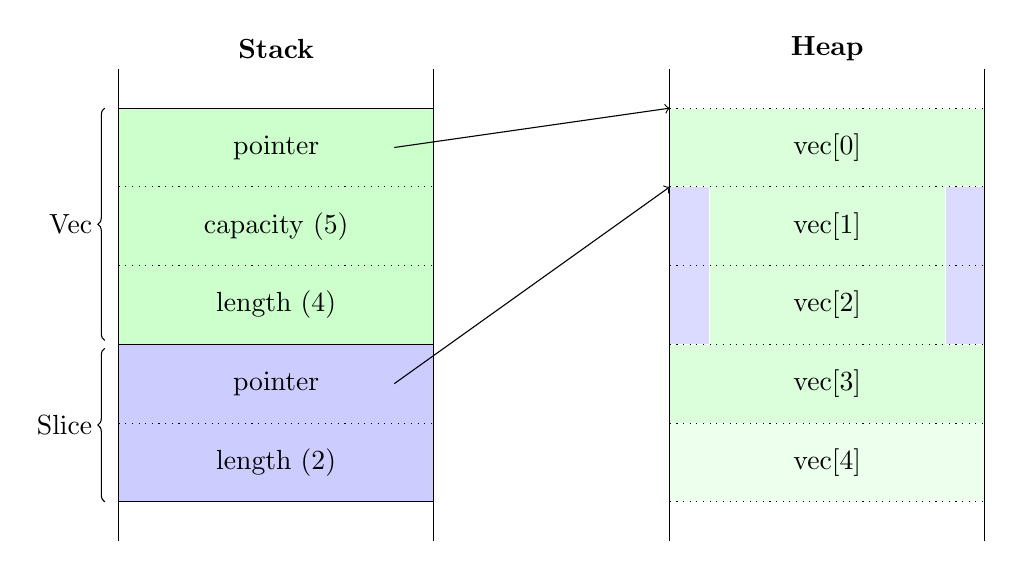
\begin{tikzpicture}
		
			\node[text width=3cm, align=center] at (3,  6.25) {\textbf{Stack}};
			\node[text width=3cm, align=center] at (10, 6.25) {\textbf{Heap}};
			
			\draw[black] (1, 0) -- (1, 6);
			\draw[black] (5, 0) -- (5, 6);
			
			\filldraw[fill=green!20!white, draw=black] (1, 5.5) rectangle(5, 2.5);
			\filldraw[fill=blue!20!white, draw=black] (1, 2.5) rectangle(5, 0.5);
			
			\draw[black, dotted] (1, 5.5) -- (5, 5.5);
			\node[text width=3cm, align=center] at (3, 5) {pointer};
			\draw[black, dotted] (1, 4.5) -- (5, 4.5);
			\node[text width=3cm, align=center] at (3, 4) {capacity (5)};
			\draw[black, dotted] (1, 3.5) -- (5, 3.5);
			\node[text width=3cm, align=center] at (3, 3) {length (4)};
			\draw[black, dotted] (1, 2.5) -- (5, 2.5);
			\node[text width=3cm, align=center] at (3, 2) {pointer};
			\draw[black, dotted] (1, 1.5) -- (5, 1.5);
			\node[text width=3cm, align=center] at (3, 1) {length (2)};
			\draw[black, dotted] (1, 0.5) -- (5, 0.5);
			
			
			% Heap
			\filldraw[fill=green!14!white, draw=black!0] (8, 5.5) rectangle(12, 1.5);
			\filldraw[fill=green!7!white, draw=black!0] (8, 1.5) rectangle(12, 0.5);
			\filldraw[fill=blue!14!white, draw=black!0] (8, 4.5) rectangle(8.5, 2.5);
			\filldraw[fill=blue!14!white, draw=black!0] (11.5, 4.5) rectangle(12, 2.5);
			
			\draw[black] (8, 0) -- (8, 6);
			\draw[black] (12, 0) -- (12, 6);
			
			
			\draw[black, dotted] (8, 5.5) -- (12, 5.5);
			\node[text width=3cm, align=center] at (10, 5) {vec[0]};
			\draw[black, dotted] (8, 4.5) -- (12, 4.5);
			\node[text width=3cm, align=center] at (10, 4) {vec[1]};
			\draw[black, dotted] (8, 3.5) -- (12, 3.5);
			\node[text width=3cm, align=center] at (10, 3) {vec[2]};
			\draw[black, dotted] (8, 2.5) -- (12, 2.5);
			\node[text width=3cm, align=center] at (10, 2) {vec[3]};
			\draw[black, dotted] (8, 1.5) -- (12, 1.5);
			\node[text width=3cm, align=center] at (10, 1) {vec[4]};
			\draw[black, dotted] (8, 0.5) -- (12, 0.5);
			
			
			
			\draw[decoration={brace,mirror,raise=5pt},decorate] (1, 5.5) -- node[left=6pt] {Vec} (1, 2.55);
			\draw[decoration={brace,mirror,raise=5pt},decorate] (1, 2.45) -- node[left=6pt] {Slice} (1, 0.5);
			
			\draw[->,black] (4.5, 5) -- (8, 5.5);
			\draw[->,black] (4.5, 2) -- (8, 4.5);
		
		\end{tikzpicture}
		\caption{Speicherlayout Vec und Slice \cite[63]{rust:orly_programming}}
		\label{rust:memory_layout:vec_slice}
	\end{figure}
	
	\item \textbf{std::boxed::Box}:
	Verweis auf einen Speicherbereich auf dem Heap für einen beliebigen Datentyp.
	Erlaubt es, u.a. Eigentümerschaft über ein unbekannt großen Datentyp zu erlangen, da dies die Größe von \textbf{Box} nicht beeinflusst (siehe \autoref{rust:generics}).
	Eine \textbf{Box} kann mit einem immer gültigen Heap-Pointer aus C und C++ verglichen werden.
	
	\item \textbf{std::string::String}: Eine UTF-8 codierte, vergrößer- und verkleinerbare Zeichenkette auf dem Heap.
	
	\item \textbf{std::rc::Rc}: Erweitert die \textbf{Box} um einen Referenzzähler und ermöglicht somit augenscheinlich mehrere Eigentümer, mit der Limitierung, nur noch lesend auf den beinhalteten Wert zugreifen zu können.
	Der beinhaltende Wert wird erst bei Lebensende der letzten \textbf{Rc} Instanz freigegeben.
	Verwendet einen mit wenig Mehraufwand verbundenen, nicht-atomaren Referenzzähler, weswegen eine \textbf{Rc} Instanz nicht zwischen Threads übertragen werden kann (\rustcinline{!Sync}, \rustcinline{!Send}).
	
	\item \textbf{std::sync::Arc}: Entspricht weitestgehend dem \textbf{Rc}, verwendet jedoch einen atomaren Referenzzähler.
	Dies ist zwar mit Mehraufwand zur Laufzeit verbunden, erlaubt aber auch, dass eine \textbf{Arc} Instanz zwischen Threads übertragen werden kann, insofern der beinhaltende Wert dies erlaubt.
	Mehrere Threads können daher lesend auf den beinhalteten Wert zugreifen.
	
	\item \textbf{std::sync::Mutex}: \todo{?} Schützt Daten anstatt Code
	\item \textbf{std::sync::RwLock}: \todo{?} Erlaubt mehrfach lesend
	\item \textbf{std::net::TcpStream}: \todo{?} 
	\item \textbf{Module std::thread}: \todo{?}
	\item \textbf{std::collections::HashMap}: \todo{?}
	
\end{itemize}


\section{Speichermanagement}
\label{rust:scope}
\label{rust:static_analysis}

Rust benutzt ein \enquote{statisches, automatisches Speicher Management -- keinen Garbage Collector} \cite{rust:youtube:goto2017}.
Das bedeutet, die Lebenszeit einer Variable wird statisch während der Compilezeit anhand des Geltungsbereichs ermittelt (siehe \autoref{rust:scope}).
Durch diese statische Analyses findet der Compiler heraus, wann der Speicher einer Variable wieder freigegeben werden muss.
Dies ist genau dann, wenn der Geltungsbereich des Eigentümers zu Ende ist.
Weder ein \gls{gc}, der dies zur Laufzeit nachverfolgt, noch ein manuelles eingreifen durch den Entwickler (zum Beispiel durch \ccinline{free(*void)}, wie in C/C++ üblich) ist nötig.

Falls der Compiler keine ordnungsgemäße Nutzung feststellen kann, wie zum Beispiel eine Referenz die länger als die eigentliche Variable lebt, wird die Kompilation verweigert.
Der menschliche Faktor als Fehlerquelle wird wieder unterbunden, ohne Laufzeitkosten zu erzeugen (siehe \autoref{rust:guarantee:no_danling_pointer}).

Im folgenden \autoref{rust:memory:scope} wird Beispielhaft Speicher auf dem Heap allokiert.
Dieser wird ordnungsgemäß freigegeben, ohne manuell eine Freigabe einzuleiten.

\begin{figure}[H]
	\rustcinclude
		{rust:memory:scope}
		{Geltungsbereich von Variablen}
		{sections/rust.memory.rs}
\end{figure}

Eine Variable kann auch vorzeitig durch den Aufruf von \rustcinline{std::mem::drop(_)} freigegeben werden.
Die optionalen Implementation des \rustcinline{std::op::Drop}-Merkmals (siehe \autoref{rust:generics}) kommt der Implementation des Destruktors aus C++ gleich.

\section{Eigentümer- und Verleihprinzip}
\label{rust:ownership}

Bereits 2003 beschreibt Bruce Powel Douglass im Buch \enquote{Real-Time Design Patterns}, dass \enquote{passive} Objekte ihre Arbeit nur in dem \todo{Thread-Kontext} ihres \enquote{aktiven} Eigentümers tätigen sollen \cite[204]{douglass2003real}.
In dem beschriebenen \enquote{Concurrency Pattern} wird eine klare Zuordnung getätigt, welche Objekte welchem anderen Objekt als Eigentümern zugeordnet sind, um eine sicherere Nebenläufigkeit zu schaffen \todo{shit}.

Diese Philosophie setzt Rust direkt in der Sprache um, so darf eine Variable immer nur einen Eigentümer haben. Zusätzlich zu einem immer eindeutig identifizierbaren Eigentümer für eine Variable, kann diese auch ausgeliehen werden; entweder exklusiv mit sowohl Lese- als auch Schreiberlaubnis, oder mehrfache mit nur Leseerlaubnis.

Eigentümerschaft kann auch übertragen werden, der vorherige Eigentümer kann danach nicht mehr auf den Wert zugreifen.

Die Garantie nur einen Eigentümer, eine exklusive Schreiberlaubnis oder mehrere Leseerlaubnisse auf eine Variable zu haben, wird durch die statische Lebenszeitanalyse garantiert (siehe \autoref{rust:scope}).
Da dies zur Compilezeit geschieht, ist eine Überprüfung zur Laufzeit nicht nötig, weshalb diese Philosophie keinen negativen Einfluss auf die \todo{Ausführgeschwindigkeit} hat.

\todo{Split example, explain more}
\rustcinclude
	{rust:ownership:scope}
	{Eigentümer und Referenzen von Variablen}
	{sections/rust.ownership.rs}


\todo{missing move? orly}


\section{Rust als funktionale Programmiersprache}
\todo{functional programming -> no global state, no exceptions, find literature}
\todo{prove via code}

\section{Rust als Objekt-Orientierte Programmiersprache}
\label{rust:oop}
\todo{trait}
\todo{prove via design patterns, a few? from faq::  Is Rust object oriented? It is multi-paradigm. Many things you can do in OO languages you can do in Rust, but not everything, and not always using the same abstraction you’re accustomed to.}


\section{Versprechen von Rust}
\label{rust:guarantees}

\begin{quotation}
	\textit{\enquote{It’s not bad programmers, it’s that C is a hostile language}} 
	\cite[54]{rust:c_is_hostile_mena}
\end{quotation}

\begin{quotation}
	\textit{\enquote{I’m thinking that C is actively hostile to writing and maintaining reliable code}} 
	\cite[129]{rust:c_is_hostile_mena}
\end{quotation}

Rust wirbt mit Versprechen und Garantien, die dafür sorgen sollen, typische Fehler zu vermeiden.
In einer perfekten Welt wären viele dieser Maßnahmen nicht nötig, da perfekte Wesen niemals einen Fehler machen würden, aber leider sind Programmierer auch nur Menschen.
Menschen, die Fehler machen.
Deswegen hat Rust einige Interessante Mechaniken eingeführt, bekannte Fehlerquellen zu unterbinden und erzwingt die Einhaltung dieser, indem andere Vorgehensweisen meist ausgeschlossen werden.

Dieses Kapitel beschäftigt sich mit den wichtigsten und bekanntesten dieser Mechaniken.

\subsection{Kein undefiniertes Verhalten}
\label{rust:no_unitialized_usage}
\label{rust:no_undefined}

Bei der Entwicklung von Rust wird ein sehr großer Fokus darauf gelegt, keine undefinierten Zustände zu erlauben.
Daher ist es normalerweise nicht möglich, ein undefiniertes Verhalten oder einen undefinierten Zustand zu erzeugen.
Die Ausnahme bildet dabei die Nutzung innerhalb von \rustcinline{unsafe} Blöcken, für zum Beispiel FFI (siehe \autoref{rust:ffi}).
Für diese Fälle gibt es eine überschaubare Liste von Szenarien, aus denen ein undefinierter Zustand bzw. undefiniertes Verhalten resultieren kann \cite{rust:book:undefined}.

Als einfaches Beispiel eines undefinierten Zustandes in C ist eine Variable, die deklariert wurde, der aber noch keinen Wert zugewiesen wurde.
In manchen Szenarien hat die Variable dann den Wert der in diesem Moment an der entsprechenden Stelle im Speicher steht, in anderen Szenarien wird der Speicher vom Betriebssystem, Allokator oder von vom Compiler eingefügten Befehlen mit 0en gefüllt -- eine sichere Aussage ist nicht möglich.

Rust lässt deshalb keinen Zugriff auf Variablen zu, die nicht zuvor initialisiert wurden \cite[126]{rust:orly_programming}.
Der Compiler stoppt mit einem Fehler: \enquote{\textbf{\textcolor{red}{error[E0381]}: use of possibly uninitialized variable: `a`}}.


\subsection{Keine vergessene Null-Pointer Prüfung}
\label{rust:no_null_detail}

\begin{quotation}
	\textit{\enquote{I call it my billion-dollar mistake. It was the invention of the null reference in 1965}}
	\cite[Tony Hoare, QCon Software Konferenz in London, 2009]{rust:infoq:null}
	\todo{cant find moment in video / presentation of this qutoe!?}
\end{quotation}

Wie in \autoref{rust:no_null} bereits erwähnt, kennt Rust keinen \ccinline{NULL}-Pointer.
Daher ist es auch nicht möglich, durch Nachlässigkeit auf den falschen Speicher zuzugreifen, da eine Referenz immer gültig ist.
Für fälle, in denen es eventuell keinen Wert gibt, bietet Rust stattdessen den \rustcinline{Option<_>} Datentyp an.
\rustcinline{Option<_>} ist eine Aufzählung, die entweder \rustcinline{None} ohne einen Wert, oder \rustcinline{Some(_)} mit einem Wert ist.
Auf den Wert kann nicht zugegriffen werden, ohne zu prüfen, ob wirklich ein \rustcinline{Some(_)} vorliegt.
Dies kann durch \rustcinline{match} oder verkürzt durch ein \rustcinline{if let Some(wert) = optional \{ /* tu etwas mit wert */ \}} geschehen (siehe \autoref{rust:match}).

In vielen fällen kann der \rustcinline{Option<_>} Datentyp in Maschinencode als \ccinline{NULL}-Pointer dargestellt werden, weswegen durch diese Abstraktion meist keine weiteren Laufzeitkosten eingeführt werden \cite[100]{rust:orly_programming} (siehe \autoref{rust:zero_cost}).



\subsection{Keine vergessene Fehlerprüfung}
\label{rust:result}

\begin{figure}[H]
	\ccinclude
	{rust:result:c_bad_fopen}
	{Negativbeispiel: Fehlende Fehlerprüfung in C}
	{sections/rust.fopen.c}
\end{figure}

In \autoref{rust:result:c_bad_fopen} sind mindestens zwei Fehler versteckt, die aber keinen Compileabbruch auslösen, sondern sich zur Laufzeit zeigen können.
Der erste Fehler ist eine fehlende Überprüfung des Rückgabewertes von \ccinline{fopen} in Zeile 4.
Der Rückgabewert kann \ccinline{NULL} sein, falls das Öffnen der Datei fehlgeschlagen ist.
Der Versuch in die Datei zu schreiben in Zeile 5 kann daraufhin in einen Speicherzugriffsfehler resultieren und das Programm abstürzen lassen.

In Rust wird weder eine Ausnahme geworfen, noch ein Rückgabewert zurück gegeben, der ohne Prüfung verwendet werden kann:

\begin{figure}[H]
	\rustcinclude
	{rust:result:rust_good_fopen}
	{Positivbeispiel: Keine fehlende Fehlerprüfung in Rust}
	{sections/rust.fopen.rs}
\end{figure}

Der Rückgabewert von \rustcinline{File::open("private.key")} in Zeile 5 von \autoref{rust:result:rust_good_fopen} ist vom Typ \rustcinline{Result<File, Error>}.
Auf den eigentlichen Rückgabewert \rustcinline{File} kann nicht ohne eine Fehlerprüfung zugegriffen werden, da dies \rustcinline{Result} verhindert.
Eine Fehlerprüfung kann wie in Zeile 5 mit einem \rustcinline{match} oder verkürzt durch ein \rustcinline{if let Ok(mut file) = ...} geschehen.

Durch die statische Lebenszeitanalyse (siehe \autoref{rust:static_analysis}) in Rust ist der Geltungsbereich der \rustcinline{File} Variable bekannt, deshalb wird in dem Beispiel in Rust in \autoref{rust:result:rust_good_fopen} die Datei auch wieder ordnungsgemäß geschlossen.
Dies ist im im C Beispiel in \autoref{rust:result:c_bad_fopen} nicht der Fall.
In einem größeren Programm könnte so zu unbekanntem Zeitpunkt das Limit an gleichzeitig geöffneten Dateien erreicht werden.


\todo{explain shorthand '?'}

\subsection{No dangling pointer}
\label{rust:guarantee:no_danling_pointer}
\todo{src https://www.youtube.com/watch?v=d1uraoHM8Gg}

\subsection{Sichere Nebenläufigkeit}

\todo{\enquote{Safety is invisible} \cite[41]{rust:orly_programming}}

\todo{Send, Sync, No dataraces weil Ownership \autoref{rust:ownership}, Channel, Mutex, RwLock}

\todo{Datarace benötigt immer einen schreibenden + min einen lesenden gleichzeitig}


\todo{Mutex, RwLock -- immer mit Result}


\subsection{Zero Cost Abstraction}
\label{rust:zero_cost}

Trotz der vielen verwendeten Abstraktionen möchte Rust dadurch möglichst keine weitere Laufzeitkosten erzeugen.
Beim übersetzen werden deshalb viele Abstraktionen durch Optimierungen für den Maschinencode unsichtbar.

Der \rustcinline{Option<_>} Datentyp kann zum Beispiel in vielen Fällen als Pointer dargestellt werden, der bei \ccinline{NULL} \rustcinline{None} und ansonsten \rustcinline{Some(_)} ist \cite[100]{rust:orly_programming}.
Somit wird eine Überprüfung erzwungen, ohne dabei Laufzeitkosten erzeugt zu haben.

Ein weiteres Beispiel sind die Referenzzählertypen \rustcinline{Rc} und \rustcinline{Arc<_>}.
Der Zähler ist im Heap direkt vor dem beinhalteten Wert und nicht in einem extra Speicherbereich, weshalb ein weiterer, indirekter Speicherzugriff mit Laufzeitkosten verhindert werden kann.


\begin{figure}[H]
	\centering
	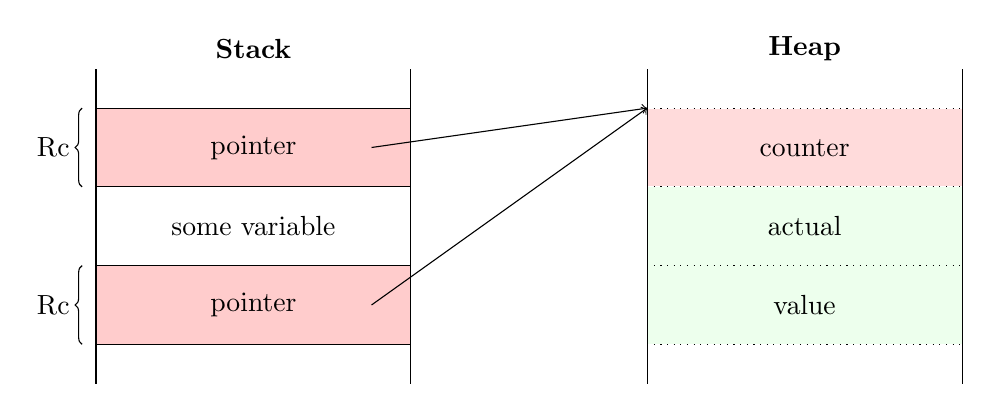
\begin{tikzpicture}
	
	\node[text width=3cm, align=center] at (3,  4.25) {\textbf{Stack}};
	\node[text width=3cm, align=center] at (10, 4.25) {\textbf{Heap}};
	
	\draw[black] (1, 0) -- (1, 4);
	\draw[black] (5, 0) -- (5, 4);
	
	\filldraw[fill=red!20!white, draw=black] (1, 3.5) rectangle(5, 2.5);
	\filldraw[fill=red!20!white, draw=black] (1, 1.5) rectangle(5, 0.5);
	%\filldraw[fill=blue!20!white, draw=black] (1, 2.5) rectangle(5, 0.5);
	
	%\draw[black, dotted] (1, 5.5) -- (5, 5.5);
	%\node[text width=3cm, align=center] at (3, 5) {pointer};
	%\draw[black, dotted] (1, 4.5) -- (5, 4.5);
	%\node[text width=3cm, align=center] at (3, 4) {capacity (5)};
	\draw[black, dotted] (1, 3.5) -- (5, 3.5);
	\node[text width=3cm, align=center] at (3, 3) {pointer};
	\draw[black, dotted] (1, 2.5) -- (5, 2.5);
	\node[text width=3cm, align=center] at (3, 2) {some variable};
	\draw[black, dotted] (1, 1.5) -- (5, 1.5);
	\node[text width=3cm, align=center] at (3, 1) {pointer};
	\draw[black, dotted] (1, 0.5) -- (5, 0.5);
	
	
	% Heap
	%\filldraw[fill=green!14!white, draw=black!0] (8, 5.5) rectangle(12, 1.5);
	\filldraw[fill=green!7!white, draw=black!0] (8, 2.5) rectangle(12, 0.5);
	\filldraw[fill=red!14!white, draw=black!0] (8, 3.5) rectangle(12, 2.5);
	%\filldraw[fill=red!14!white, draw=black!0] (11.5, 3.5) rectangle(12, 2.5);
	
	\draw[black] (8, 0) -- (8, 4);
	\draw[black] (12, 0) -- (12, 4);
	
	
	%\draw[black, dotted] (8, 5.5) -- (12, 5.5);
	%\node[text width=3cm, align=center] at (10, 5) {vec[0]};
	%\draw[black, dotted] (8, 4.5) -- (12, 4.5);
	%\node[text width=3cm, align=center] at (10, 4) {vec[1]};
	\draw[black, dotted] (8, 3.5) -- (12, 3.5);
	\node[text width=3cm, align=center] at (10, 3) {counter};
	\draw[black, dotted] (8, 2.5) -- (12, 2.5);
	\node[text width=3cm, align=center] at (10, 2) {actual};
	\draw[black, dotted] (8, 1.5) -- (12, 1.5);
	\node[text width=3cm, align=center] at (10, 1) {value};
	\draw[black, dotted] (8, 0.5) -- (12, 0.5);
	
	
	
	\draw[decoration={brace,mirror,raise=5pt},decorate] (1, 3.5) -- node[left=6pt] {Rc} (1, 2.5);
	\draw[decoration={brace,mirror,raise=5pt},decorate] (1, 1.5) -- node[left=6pt] {Rc} (1, 0.5);
	%\draw[decoration={brace,mirror,raise=5pt},decorate] (1, 2.45) -- node[left=6pt] {Slice} (1, 0.5);
	
	%\draw[->,black] (4.5, 5) -- (8, 5.5);
	\draw[->,black] (4.5, 3) -- (8, 3.5);
	\draw[->,black] (4.5, 1) -- (8, 3.5);
	
	\end{tikzpicture}
	\caption{Speicherlayout Rc \cite[90-91]{rust:orly_programming}}
\end{figure}



\section{Einbinden von Bibliotheken}

\subsubsection{Externe Datentypen}
\label{rust:ffi}
\label{rust:ffi:datatypes}

Rust bietet durch das \gls{ffi} die Möglichkeit, andere (System-)Bibliotheken einzubinden.
Entsprechende Strukturen und Funktionen werden durch einen \rustcinline{extern} Block
oder im Falle von Strukturen stattdessen optional mit einem \rustcinline{#[repr(C)]} gekennzeichnet.

In einem Beispiel, soll die Nutzung von \gls{ffi} demonstriert werden.

\begin{figure}[H]
	\ccinclude
		{rust:ffi:position_offset_c}
		{Ausschnitt von \enquote{PositionOffset} (C-Code) aus der \textit{libmessages-sys} Crate}
		{sections/rust.position_offset.c}
	
\end{figure}

Die Struktur in \autoref{rust:ffi:position_offset_c} muss zur Nutzung in Rust zuerst bekannt gemacht werden.
Dabei gibt es mehrere Möglichkeiten:
\begin{itemize}
	\item Falls der Aufbau der Struktur nicht von Bedeutung ist, kann es ausreichen, den Datentyp lediglich bekannt zu machen: \rustcinline{#[repr(C)] struct PositionOffset;}.
	In diesem Fall können aber nur Referenzen und Raw-Pointer auf die Struktur verwendet werden.
	\label{rust:ffi:example:enumerate:repr}
	
	\item Falls der Aufbau wie in \autoref{rust:ffi:example:enumerate:repr} unbedeutend ist, es soll aber ausdrücklich auf einen externen Datentyp hingewiesen werden, kann dieser in einem \rustcinline{extern \{ \} } Block bekannt gemacht werden: \rustcinline{extern \{ type PositionOffset; \}} \cite{rust:github:extern_type}.
	Dies ist zum jetzigen Zeitpunkt aber nur in \enquote{nightly} und hinter dem \enquote{feature gate} \monospaceinline{extern_types} möglich.
	
	\item Der Inhalt der Struktur ist von Bedeutung, da darauf zugegriffen oder in Rust eine Instanz werden soll. In diesem Fall ist eine komplette Wiedergabe die Struktur unumgänglich:
	\begin{figure}[H]
		\rustcinclude
			{rust:ffi:position_offset_rust}
			{Ausschnitt von \enquote{PositionOffset} (Rust-Code) aus der \textit{libmessages-sys} Crate}
			{sections/rust.position_offset.rs}
	\end{figure}
	
	In \autoref{rust:ffi:position_offset_rust} ist die Struktur \enquote{PositionOffset} deklariert,
	die durch das Attribut \rustcinline{#[repr(C)]} wie eine C-Struktur im Speicher organisiert wird.
	Damit die Struktur in Rust kompatibel zu der in C ist, müssen die Variablen von der selben Größe sein, ansonsten würde das Speicherlayout nicht übereinstimmen.
	Hierfür werden spezielle Datentypen (\rustcinline{c_long}, \rustcinline{c_void}, \rustcinline{c_char}, ...) angeboten, um die Kompatibilität mit verschiedenen Systemen und C-Compilern zu wahren.
	% (siehe \autoref{rust:types:simple}).
	
%	\rustcinline{*mut c_long} entspricht dabei dem C-Pointer für \rustcinline{&mut c_long}, also \ccinline{long*}, ein C-Pointer für \rustcinline{&c_long} entspricht \rustcinline{*const c_long}.
	
%	C-Pointer werden in Rust \enquote{Raw-Pointer} genannt und \rustcinline{*mut c_long} für  \rustcinline{&mut c_long} bzw. \rustcinline{*const c_long} für \rustcinline{&c_long} geschrieben.
	
	Ein C-Pointer \ccinline{*long} wird in Rust \enquote{Raw-Pointer} genannt und entweder \rustcinline{*mut c_long} oder \rustcinline{*const c_long} geschrieben. Der Unterschied ist wie zwischen \rustcinline{&mut c_long} und \rustcinline{&c_long} und dient dem Rust Compiler zum Nachvollziehen, ob ein exklusiver zugriff benötigt wird, oder nicht.
	Dies hilft zwar für die Fehlervermeidung durch eventuelle Compilefehler anstatt Laufzeitfehler, ist aber für die C-Funktion unbedeutend \cite{rust:book:raw_ptr}:
	
	\begin{figure}[H]
		\centering
		\begin{tabular}{c|c|c}
			Referenz in Rust & Raw-Pointer in Rust & C-Pointer \\
			\hline
			\rustcinline{&mut c_long}  &   \rustcinline{*mut   c_long}  &   \ccinline{long*} \\
			\rustcinline{    &c_long}  &   \rustcinline{*const c_long}  &   \ccinline{long*}
		\end{tabular}
		\caption{Vergleich Rust Raw-Pointer und Referenz zu C-Pointer}
	\end{figure}
	
\end{itemize}

\subsubsection{Externer Funktionsaufruf}
\label{rust:ffi:functioncall}

Externe Funktionen müssen im Gegensatz zu externen Strukturen immer in einem \rustcinline{extern \{\}} Block deklariert sein.

\begin{figure}[H]
	\rustcinclude
		{rust:ffi:uper_encode_to_buffer}
		{Externe Funktionsdefinition der ASN.1 Funktion zum Enkodieren}
		{sections/rust.uper_encode_to_buffer.rs}
\end{figure}

Wie in \autoref{rust:ffi:uper_encode_to_buffer} zu sehen ist, können auch \rustcinline{extern \{\}} Blöcke mit Attributen versehen werden. Zwingend ist bei der Verwendung eines \rustcinline{#[link(..)]} Attributes der Name der Bibliothek, auf die sich der im \rustcinline{extern \{\}} Block stehende Code bezieht. Optional kann auch wie in \autoref{rust:ffi:uper_encode_to_buffer} die Art der Linkung (dynamisch oder statisch) angegeben werden.

Die Art der Definition einer externen Funktion unterscheidet sich nicht von einer normalen Funktionsdefinition. Es sollten aber, wie in \autoref{rust:ffi:datatypes} beschrieben, zu C bzw. der externen Sprache kompatiblen Datentypen verwendet werden.
 


\section{Kernfeatures}

\todo{nothing on heap unless specified (Box, Vec, other container)}

\todo{closures are fast, orly, p.310}

https://www.youtube.com/watch?v=d1uraoHM8Gg \\
\todo{no need for a runtime, all static analytics} \\
\todo{memory safety} \\
\todo{data-race freedom} \\
\todo{active community} \\
\todo{concurrency: no undefined behavior} \\
\todo{ffi binding} \gls{ffi} \\
\todo{zero cost abstraction} \\
\todo{package manager: cargo} \\

https://www.youtube.com/watch?v=-Tj8Q12DaEQ \\
\todo{static type system with local type inference } \\
\todo{explicit notion of mutability } \\
\todo{zero-cost abstraction *(do not introduce new cost through implementation of abstraction)} \\
\todo{errors are values not exceptions}
\todo{no null} \\
\todo{"static automatic memory management" - no garbage collection } \\
\todo{often compared to GO and D (~44min)} \\


\section{Schwächen}

https://www.youtube.com/watch?v=-Tj8Q12DaEQ \\
\todo{compile-times} \\
\todo{Rust is a vampire language, it does not reflect at all!} \\
\todo{depending on the field -> majority of libraries?} \\


\section{Performance Fallstricke}

\todo{\cite{rust:performance_pitfalls}}

\section{Beispiele von Verwendung von Rust}

\todo{firefox} \\

https://www.youtube.com/watch?v=-Tj8Q12DaEQ \\
\todo{GTK binding heavily to rust} \\

\todo{unstable}
\todo{ffi}
